\chapter{On the production of entangled beams from a metastable Helium BEC}
\label{Peaks}
\graphicspath{{Figures/Peaks/}}

The results presented in this chapter have been published in \citet{Dall:2009}. All of the theoretical work in this paper except as noted in this chapter was my own work.

\section{Introduction}
Sources of matter waves gained a dramatic improvement with the achievement of Bose-Einstein condensation (BEC) in dilute gases and the development of the atom laser \citep{Anderson:1995vn,Mewes:1997}. Like optical lasers before them, atom lasers can produce Heisenberg-limited beam profiles \citep{Busch:2002zr,Riou:2006uq} and promise high spectral density through their dramatically lower linewidth \citep{Wiseman:1997ba}. Another exciting possibility resulting from having such a coherent source of atoms is the generation of nonclassical matter waves through entangled beams. Such entangled beams are useful for tests of quantum mechanics and are required to perform Heisenberg-limited interferometry \citep{Dowling:1998,Reid:1988}. In this chapter, we show that the asymmetric scattering lengths between internal states of metastable helium (He*) cause well-defined peaks in the output of an atom laser. These peaks are due to a phase-matched four-wave mixing (FWM) process and are experimentally demonstrated.

A nonlinear process is required to produce entanglement, and one of the advantages of atomic systems over optical systems is that there are strong inherent nonlinearities due to atomic interactions, although these interactions can also lead to complications. These nonlinearities allow certain analogues of nonlinear optical experiments such as four-wave mixing (FWM) and Kerr squeezing to be performed directly in the atomic sample \citep{WallsMilburn}. All of these produce entanglement in optical systems. Four-wave mixing in a trapped BEC has been demonstrated experimentally in configurations where three distinct momentum states generated a fourth \citep{Deng:1999qy} and where two momentum states generated a pair of correlated atomic beams \citep{Vogels:2002}. These experiments demonstrated that the output phase was coherent, but the correlation properties were not measured. More recently the pair correlations in a spontaneous scattering of two colliding condensates were measured using the single-atom detectors available for He* atoms \citep{Perrin:2007}.

Using these existing sources of entangled pairs of atoms for interferometric experiments will be complicated by the high densities of the sources, where the nonlinearities that generated the correlations ultimately degrade the long-term coherence of the sample. While recent experiments have increased the coherence of atom interferometers by several orders of magnitude by reducing the nonlinearities with a Feschbach resonance \citep{Fattori:2008,Gustavsson:2008}, this precludes the production of entangled pairs. In our scheme the nonlinear interactions are used to drive FWM in the magnetically untrapped condensate, but the resulting untrapped beams that propagate in free space are dilute, potentially avoiding the decoherence problem. We show that pairs of beams can be produced simply by the process of radio-frequency (rf) outcoupling from a He* BEC, without the need for Feschbach resonances, optical traps, or scattering pulses. Unlike previous methods, which required pairs of atoms travelling at high kinetic energies as a source, this process involves scattering between atoms initially in the same zero-momentum state to create states with nonzero momentum. Semiclassical and field-theoretic simulations of the experiment show that the beams are generated by the same FWM process that generated entangled atom pairs in the earlier experiments.

\section{The metastable Helium `Peaks' experiment}
\label{Peaks:ExperimentalSetup}

The experimental setup for creating He* BEC has been reported elsewhere \citep{Dall:2007a}, and discussed earlier in this thesis (see \sectionref{He*Experiment}\footnote{FIXME: Correct this reference when this section is written}).

Starting from an almost pure BEC containing up to $5\times 10^6$ atoms an atom laser beam was created by using rf photons to spin flip the BEC atoms from the $m=1$ magnetically trapped state to the $m=0$ untrapped state.

After outcoupling, atoms in the atom laser beam fell under gravity for a distance of $\unit[4]{cm}$ until they hit a double stacked multichannel plate (MCP). The phosphor screen was imaged with a charge-coupled-device (CCD) camera with a resolution of approximately $\unit[150]{\micro m}$ at the MCP. To remove any nonuniformities caused by spatial variations in the gain of the MCP, all images were divided by a flat-field image produced by dropping atoms from a MOT onto the detector. Since the MOT temperature is of order $\sim\unit[1]{mK}$, the spatial profile of the MOT uniformly illuminates the MCP. Although $m=-1$ atoms are produced by the outcoupling, especially for high rf powers, they are in general accelerated away from the detector by the magnetic trap field. Those that are accelerated towards the detector do not show up in the images since they arrive much earlier than the CCD trigger time.

\figureref{Peaks:ExperimentalResults} shows the dramatic change in the atom laser spatial profile when the condensate undergoes the resonant FWM process. In the case of low outcoupling Rabi frequencies (upper row), the FWM process does not occur and we see the usual double-peaked He*-atom laser profile \citep{Dall:2007} (see also \sectionref{TransverseProfile:Helium}\footnote{FIXME: Correct this reference when this section is written}). When the Rabi frequencies are high enough to initiate the FWM process (lower row), the atoms in the atom laser beam are scattered to form a halo around the main atom laser beam. Due to conservation of energy, the outer diameter of this halo corresponds to a maximum kinetic energy given by the chemical potential. As well as the ring structure, four peaks are observed on the outskirts of the profile.
% Each peak contains 11\%--14\% of the total outcoupled atoms, in agreement with the value of 11\% obtained from the simulation results shown in the lower row of \figureref{Peaks:ExperimentalResults}.

These peaks arise from two momentum-correlated cones of particles scattering out of the condensate and falling to the detector, as shown in \figureref{Peaks:Schematic}. The cones themselves are generated by a dynamical instability that populates momentum modes lying along the weak trapping axis, which expand to rings due to the mean-field repulsion in the tight trapping direction as they leave the BEC. Atoms in these cones then fall under gravity onto the detector, where the time-integrated flux is converted to a spatial density distribution, and each momentum ring appears as a double peak. The background halo is produced during the initial switch-on of the atom laser during which the peaks produced by the FWM process sweep in position from the main atom laser profile towards their final position in \figureref{Peaks:ExperimentalResults}.

\begin{figure}[htbp]
    \centering
        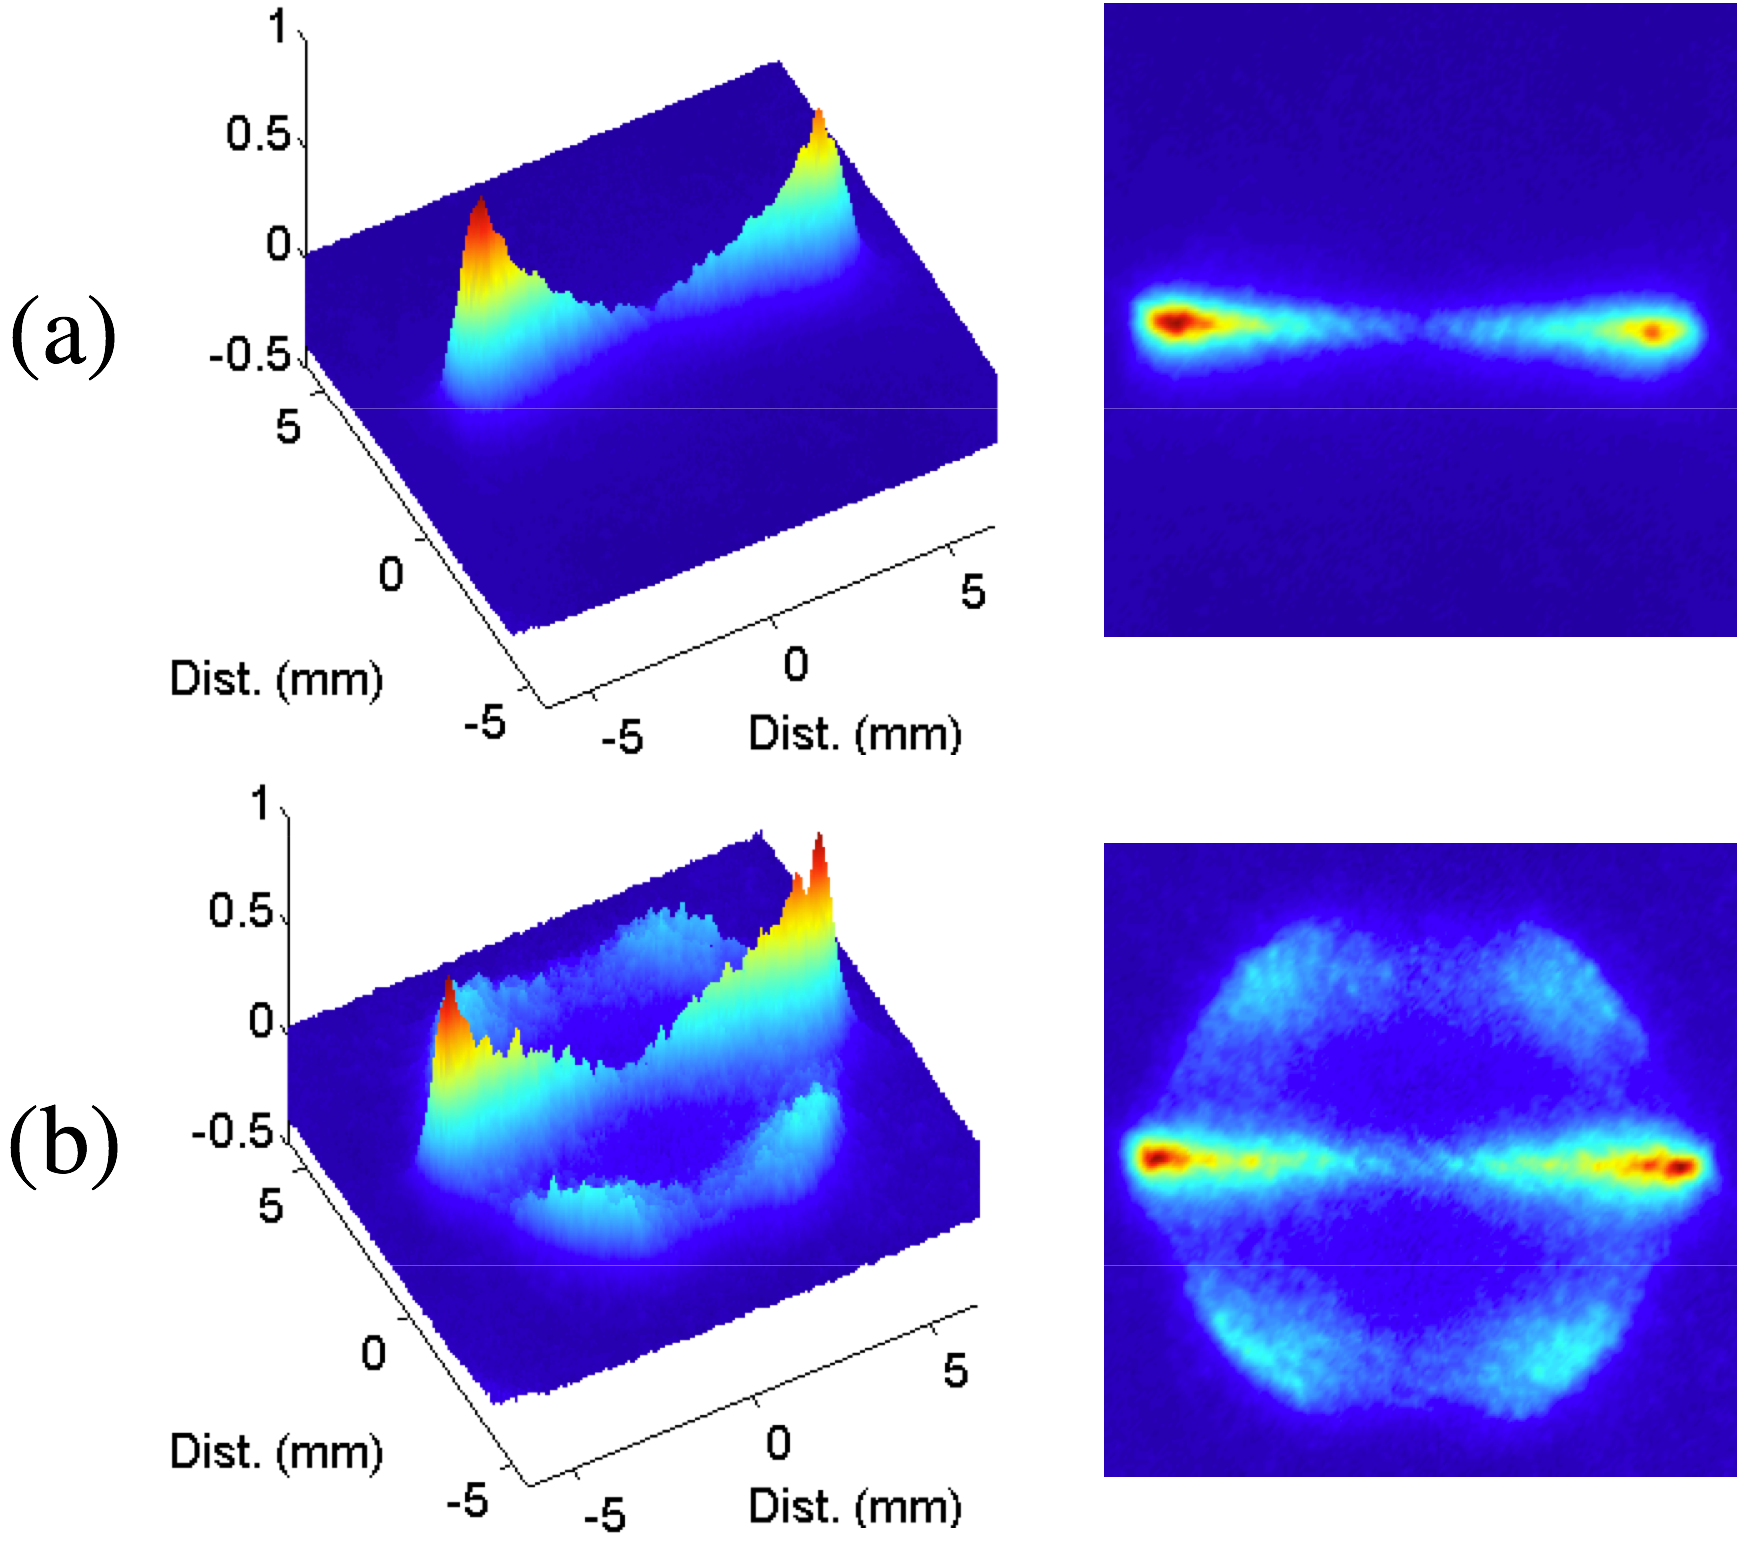
\includegraphics[height=3in]{ExperimentalResults}
    \caption{Experimental results. The difference between (a) and (b) is that the outcoupling Rabi frequency has been increased by an order of magnitude in (b).}
    \label{Peaks:ExperimentalResults}
\end{figure}

\begin{figure}[htbp]
    \centering
        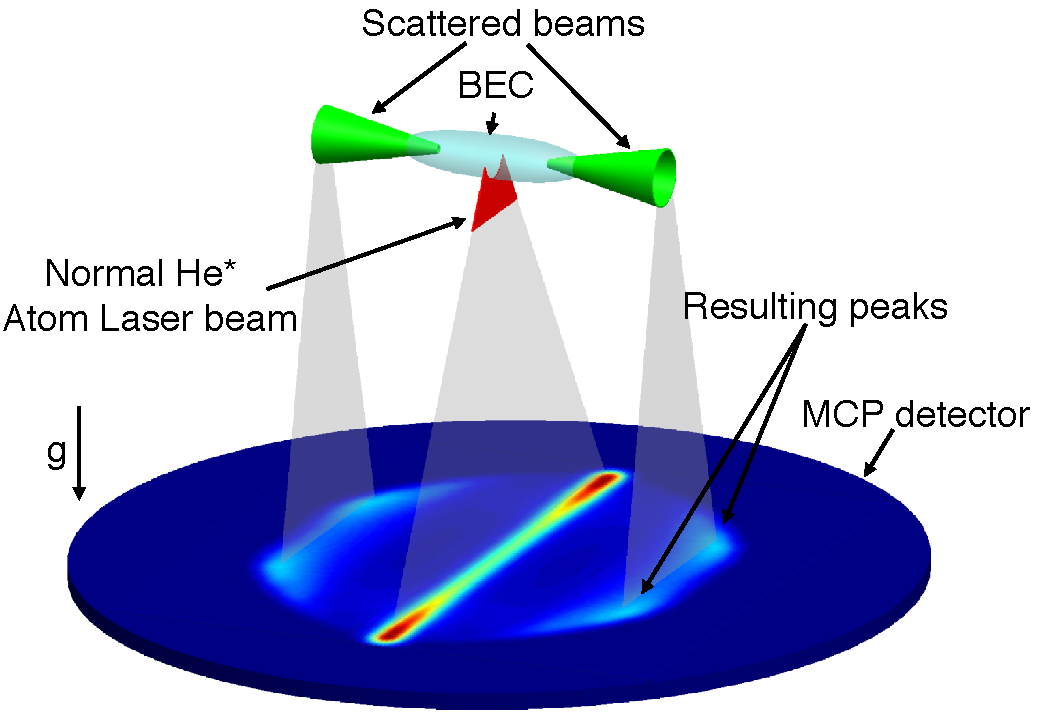
\includegraphics[height=3in]{Schematic}
    \caption{Schematic of the experimental setup}
    \label{Peaks:Schematic}
\end{figure}


\begin{table}
    \centering
    \begin{tabular}{cc}
    \toprule
    Parameter & Value\\
    \midrule
    Condensate number & $N = 2\times 10^6$\\
    Radial trapping frequency & $\omega_\rho = 2 \pi \times \unit[1020]{Hz}$\\
    Axial trapping frequency & $\omega_z = 2\pi \times \unit[55]{Hz}$\\
    Outcoupling Rabi frequency & $\Omega = 2\pi \times \unit[3]{kHz}$\\
    \bottomrule
    \end{tabular}
    \caption{Experimental parameters for the metastable Helium BEC under consideration.}
    \label{Peaks:ExperimentalParameters}
\end{table}

\section{Semianalytic treatment}

%While the argument in the previous section gives a qualitative explanation for the four-wave mixing process observed in He*, it is not entirely satisfying. In this section an approximate analytic expression for the excited modes of the He* system will be obtained and investigated using Bogoliubov stuff.

The observed peaks in the atom laser profile presented in the previous section are caused by a dynamical instability in the condensate that causes the formation of momentum excitations in a narrow range of momenta along the weak trapping axis.
% The background halo between these peaks and the usual atom laser profile is the result of (at higher detunings resonant momentum will vary across surfaces, during this initial switch-on phase, a range of momenta are excited)\footnote{FIXME: Complete and correct this sentence.}.
This effect is due to the significantly different scattering lengths between the Zeeman levels of He*. In a later section a full multimode quantum-field calculation will be discussed and its results presented, but it is enlightening to first consider a simplified model in which the energy spectrum (and stability) of small excitations to the condensate can be obtained.

The simplified model to be considered is that of a homogenous spinor condensate consisting of two levels with Rabi oscillations coupling the two levels. The approximation that the condensate is homogenous (known as the local density approximation \cite{Stamper-Kurn:1999,Zambelli:2000}) is justified if the excitations under considerations have wavelengths much smaller than the Thomas-Fermi radius in that dimension. The local density approximation will hold for this system along the axial direction as the axial momentum of the features observed in \figureref{Peaks:ExperimentalResults} corresponds to an excitation wavelength of $\sim \unit[5]{\micro m}$, significantly smaller than the Thomas-Fermi radius in the axial direction of $z_\text{TF} = \unit[175]{\micro m}$. 

The second approximation made in this model is to neglect the antitrapped state $m_F=-1$. Any density in this state leaves the condensate very rapidly due to the combined effects of both the mean-field repulsion and the magnetic field gradient. A classical particle in the centre of the condensate under the influence of the same effective potential experienced by the $m_F=-1$ atoms would leave the condensate in $\sim \unit[80]{\micro s}$, significantly shorter than the inverse Rabi frequency of $\sim \unit[300]{\micro s}$.

With these approximations made, the Hamiltonian for this system is
\begin{align}
    \begin{split}
    \hat{H} &= \sum_i \int d\mathbf{x}\, \hat{\Psi}_i^\dagger \left(\frac{-\hbar^2 \nabla^2}{2 M} - \mu\right)\hat{\Psi}_i^{} + \frac{1}{2} \sum_{i j} U_{i j}\int d\mathbf{x}\, \hat{\Psi}_i^\dagger \hat{\Psi}_j^\dagger \hat{\Psi}_j^{} \hat{\Psi}_i^{}\\
            &\phantom{=} + \hbar \Omega \int d\mathbf{x}\, \left(\hat{\Psi}_1^\dagger \hat{\Psi}_0^{} + \hat{\Psi}_0^\dagger \hat{\Psi}_1^{}\right),
    \end{split}
\end{align}
where $U_{ij} = 4\pi \hbar^2 a_{ij}/M$ is the nonlinear interaction strength, $a_{ij}$ is the s-wave scattering length between internal states $i$ and $j$, and $\Omega$ is the Rabi frequency which is taken to be real. The equations of motion corresponding to this Hamiltonian are
\begin{subequations}
    \label{Peaks:OperatorEquationsOfMotion}
    \begin{align}
    i \hbar \frac{\partial \hat{\Psi}_1}{\partial t}  &= -\frac{\hbar^2}{2M}\nabla^2 \hat{\Psi}_1  + U \left(\hat{\Psi}_1^\dagger \hat{\Psi}_1^{} + \hat{\Psi}_0^\dagger \hat{\Psi}_0^{}\right) \hat{\Psi}_1^{} + \hbar \Omega \hat{\Psi}_0^{},  \\
    i \hbar \frac{\partial \hat{\Psi}_0}{\partial t} &= -\frac{\hbar^2}{2M} \nabla^2 \hat{\Psi}_0 + U \left(\hat{\Psi}_1^\dagger \hat{\Psi}_1^{} + \kappa \hat{\Psi}_0^\dagger \hat{\Psi}_0^{} \right) \hat{\Psi}_0^{} + \hbar \Omega \hat{\Psi}_1^{},
    \end{align}
\end{subequations}
where $U=U_{11}=U_{10}$ and $\kappa = U_{00}/U_{11}$. For metastable Helium in the $F=1$ manifold, $\protect{\kappa \approx 0.74}$\footnote{FIXME: Cite something.}, while for Rubidium in the $F=1$ manifold, $\kappa \approx 1.01$ \cite{Ho:1998}\footnote{FIXME: A more recent reference might be useful.}. 

\subsection{The dynamical steady-state}

The excitation spectrum of a condensate can be obtained by approximating each field operator to be a c-number (the mean-field) plus a small fluctuation term, and then either diagonalising the Hamiltonian \cite{Bogoliubov:1947,FetterWalecka} or diagonalising the linearised equations of motion for the fluctuations themselves (see, for example \cite{Ho:1998}\footnote{FIXME: Probably need an earlier and/or better reference here.}). It is the latter approach that will be taken here, but with the difference that the mean-field about which the linearisation procedure will take place is itself time-dependent.

The mean-field state that we wish to consider is one that corresponds to the state of the BEC in the experiment. At $t=0$ all of the population in this state will be in the $m_F=1$ level, representing the original trapped BEC, while the $m_F=0$ atom laser level will be initially unpopulated. Rabi oscillations will transfer population between these two levels, and it will be shown that these oscillations are periodic.

The method for diagonalising the evolution equations of the linearised fluctuations to obtain the excitation spectrum is the same method used to determine the stability of fixed points of systems of nonlinear ordinary differential equations. This method relies critically on the fact that it is a \emph{fixed} point about which the equations are linearised. Floquet's Theorem\footnote{FIXME: Cite some random ODE text.} allows the stability of \emph{periodic} solutions to be considered, and it is this theorem that will be used to determine the stability of the mean-field evolution. It now remains to be shown that this mean-field evolution is periodic.

Within the local density approximation we can assume that the mean-field remains homogeneous; only the excitations will have spatial dependence. The equations of motion for the mean-field then reduce to the following ordinary differential equations,
\begin{subequations}
    \label{Peaks:MeanFieldEquationsOfMotion}
    \begin{align}
    i \hbar \frac{d \Psi_1}{dt} &= U\left(\abs{\Psi_1}^2 + \abs{\Psi_0}^2\right)\Psi_1 + \hbar \Omega \Psi_0,\\
    i \hbar \frac{d \Psi_0}{dt} &= U\left(\abs{\Psi_1}^2 + \kappa \abs{\Psi_0}^2\right)\Psi_0 + \hbar \Omega \Psi_1.
    \end{align}
\end{subequations}

Although solving \eqref{Peaks:MeanFieldEquationsOfMotion} for $\kappa \neq 1$ is intractable analytically, it can at least be shown that the solutions are periodic. This can be shown by recognising these equations as modified optical Bloch equations containing a nonlinear term but with no damping. Defining $\Psi_i = c_i\sqrt{n}$ where $n = \abs{\Psi_1}^2 + \abs{\Psi_0}^2$ is the total density, the equations of motion for the density matrix terms $\rho_{10} = c_{1}^{}c_{0}^*$ and $w = \rho_{11}-\rho_{00} = \abs{c_1}^2 - \abs{c_0}^2$ are
\begin{subequations}
    \label{Peaks:OpticalBlochEquations}
    \begin{align}
        \frac{d\rho_{10}}{dt} &= -i\frac{g}{2} (1-w)\rho_{10} + i \Omega w,\\
        \frac{d w}{dt} &= -4 \Omega \Im\{\rho_{10}\},
    \end{align}
\end{subequations}
where $g = n U (1-\kappa)/\hbar$. As the evolution is purely Hamiltonian, these equations will conserve the energy of the state. Up to an arbitrary additive constant, this energy is given by
\begin{align}
    E &= -\frac{1}{8}\hbar g(1 - w)^2 + 2 \hbar \Omega \Re\{\rho_{10}\}.
    \label{Peaks:OpticalBlochEnergy}
\end{align}
The solutions to \eqref{Peaks:OpticalBlochEquations} are visualised in \figureref{Peaks:BlochSphere}.

As the evolution is purely Hamiltonian, the state can be described by a point on the surface of the Bloch sphere (see \figureref{Peaks:BlochSphere}).  The state is however not completely free to move on this sphere as the Hamiltonian must be conserved by its motion. This further restricts the system's motion to closed lines on the surface of the Bloch sphere, therefore requiring the system's motion to be periodic. It is this periodicity that will enable the stability of the condensate to excitations to be determined.

\begin{figure}
    \centering
    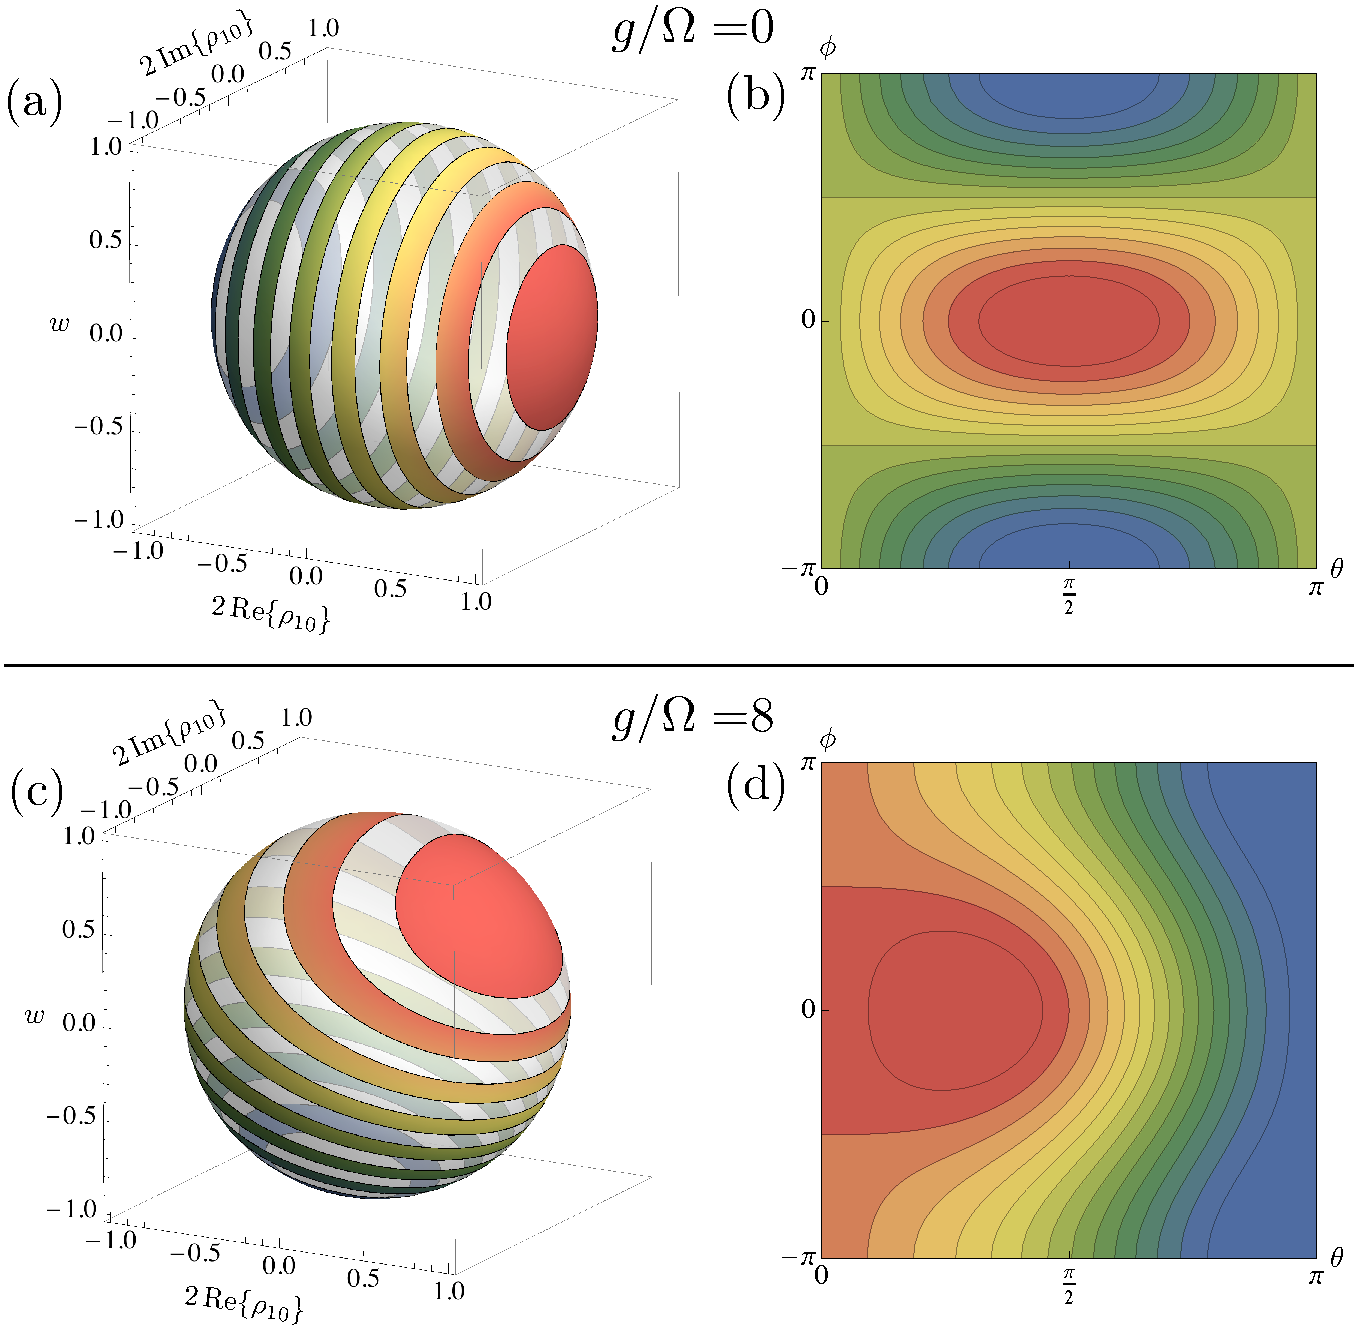
\includegraphics[width=14cm]{BlochSpheres}
    \caption{Bloch sphere representation of the evolution described by \eqref{Peaks:OpticalBlochEquations}. The upper figures (a) and (b) represent the case of the usual optical Bloch equations without any damping ($g/\Omega=0$), the lower figures (c) and (d) illustrate the effect of the nonlinear term in the evolution with $g/\Omega = 8$. The left figures (a) and (c) illustrate the Bloch sphere shaded with colour depending on the energy $E$ [see \eqref{Peaks:OpticalBlochEnergy}]. The system is constrained to move on lines of constant colour. Bands have been removed from these spheres for illustration purposes only. The right figures (b) and (d) are contour plots of the energy $E$ over the surface of the Bloch sphere.
     \label{Peaks:BlochSphere}}
\end{figure}

\subsection{Excitation dynamics}

The evolution of small perturbations about the mean-field dynamics of a condensate define both the excitation spectrum of the condensate and its stability to perturbations. 
%These perturbations not only arise from experimental uncertainties, but are an  inescapable consequence of quantum mechanics due to the fluctuations of the vacuum itself.
To determine the evolution of these excitations the mean-field dynamics must be separated from that of the excitations. To this aim we define the deviation operators $\delta\hat{\Psi}_i = \hat{\Psi}_i - \mean{\hat{\Psi}_i}$ and treat $\delta\hat{\Psi}_i$ as a small quantity. In this case the $\mean{\hat{\Psi}_i}=\Psi_i$ are themselves time dependent, obeying the equations for the mean-field, \eqref{Peaks:MeanFieldEquationsOfMotion}.

The equations of motion for the deviation operators are obtained by replacing the field operators $\hat{\Psi}_i$ in the operator evolution equations \eqref{Peaks:OperatorEquationsOfMotion} and keeping only terms up to first order in the deviation operators. Applying this procedure and moving into a rotating frame to remove the global rotation in phase due to the chemical potential $\mu$ gives
\begin{subequations}
    \label{Peaks:DeviationOperatorsEvolutionXSpace}
    \begin{align}
        \begin{split}
            i \hbar \frac{\partial \delta \hat{\Psi}_1}{\partial t} =& U\left[ \left(2\abs{\Psi_1}^2+\abs{\Psi_0}^2 \right)\delta \hat{\Psi}_1 + \Psi_1^2\delta\hat{\Psi}_1^\dagger + \Psi_1\Psi_0\delta\hat{\Psi}_0^\dagger + \Psi_0^*\Psi_1\delta\hat{\Psi}_0\right]\\
                    & - \frac{\hbar^2}{2M}\nabla^2 \delta \hat{\Psi}_1 +\hbar \Omega\delta\hat{\Psi}_0- \mu \delta \hat{\Psi}_1,
        \end{split}\\
        \begin{split}
        i \hbar \frac{\partial \delta \hat{\Psi}_0}{\partial t} =& U\left[\left(2\kappa \abs{\Psi_0}^2 +\abs{\Psi_1}^2\right)\delta\hat{\Psi}_0 + \kappa \Psi_0^2 \delta\hat{\Psi}_0^\dagger + \Psi_1\Psi_0\delta\hat{\Psi}_1^\dagger + \Psi_1^*\Psi_0\delta\hat{\Psi}_1\right]\\
                    & -\frac{\hbar^2}{2M}\nabla^2 \delta \hat{\Psi}_0 +\hbar \Omega\delta\hat{\Psi}_1 - \mu \delta\hat{\Psi}_0.
        \end{split}
    \end{align}
\end{subequations}

Having assumed the condensate to be homogenous, the system is translation-invariant and the evolution equations will take their simplest form in a Fourier basis. Performing the Fourier transform of \eqref{Peaks:DeviationOperatorsEvolutionXSpace} yields
\begin{subequations}
    \label{Peaks:DeviationOperatorsEvolutionKSpace}
    \begin{align}
        \begin{split}
            i \hbar \frac{\partial \delta \hat{\Psi}_1(\mathbf{k})}{\partial t} =& U\left[ \left(2\abs{\Psi_1}^2+\abs{\Psi_0}^2 \right)\delta \hat{\Psi}_1(\mathbf{k}) + \Psi_1^2\delta\hat{\Psi}_1^\dagger(-\mathbf{k}) + \Psi_1\Psi_0\delta\hat{\Psi}_0^\dagger(-\mathbf{k}) + \Psi_0^*\Psi_1\delta\hat{\Psi}_0(\mathbf{k})\right]\\
                    & - \frac{\hbar^2 \mathbf{k}^2}{2M} \delta \hat{\Psi}_1(\mathbf{k}) +\hbar \Omega\delta\hat{\Psi}_0(\mathbf{k})- \mu \delta \hat{\Psi}_1(\mathbf{k}),
        \end{split}\\
        \begin{split}
        i \hbar \frac{\partial \delta \hat{\Psi}_0(\mathbf{k})}{\partial t} =& U\left[\left(2\kappa \abs{\Psi_0}^2 +\abs{\Psi_1}^2\right)\delta\hat{\Psi}_0(\mathbf{k}) + \kappa \Psi_0^2 \delta\hat{\Psi}_0^\dagger(-\mathbf{k}) + \Psi_1\Psi_0\delta\hat{\Psi}_1^\dagger(-\mathbf{k}) + \Psi_1^*\Psi_0\delta\hat{\Psi}_1(\mathbf{k})\right]\\
                    & -\frac{\hbar^2 \mathbf{k}^2}{2M} \delta \hat{\Psi}_0(\mathbf{k}) +\hbar \Omega\delta\hat{\Psi}_1(\mathbf{k}) - \mu \delta\hat{\Psi}_0(\mathbf{k}).
        \end{split}
    \end{align}
\end{subequations}

In this form, it is clear that the Fourier modes are almost completely decoupled from each other. Each deviation operator $\delta\hat{\Psi}_i(\mathbf{k})$ is only coupled to $\left\{\delta\hat{\Psi}_j(\mathbf{k}),\, \delta\hat{\Psi}_j^\dagger(-\mathbf{k})\right\}$, with the $\delta\hat{\Psi}_i^\dagger(-\mathbf{k})$ also only coupled to this same set. This can be exploited to write the equations \eqref{Peaks:DeviationOperatorsEvolutionKSpace} in matrix form as
\begin{align}
    i \hbar \frac{\partial \hat{\Upsilon}(\mathbf{k})}{\partial t} &= \mathcal{H}(\mathbf{k}) . \hat{\Upsilon}(\mathbf{k}),
\end{align}
where
\begin{align}
    \hat{\Upsilon}(\mathbf{k}) &= 
    \begin{pmatrix}
        \delta\hat{\Psi}_1(\mathbf{k}) &
        \delta\hat{\Psi}_1^\dagger(-\mathbf{k}) &
        \delta\hat{\Psi}_0(\mathbf{k}) &
        \delta\hat{\Psi}_0^\dagger(-\mathbf{k})
    \end{pmatrix}^T,\\
    \mathcal{H}(\mathbf{k}) &=
    \begin{pmatrix}
        \varepsilon(\mathbf{k}) + q_{1} - \mu & v_{11} & u_{01} + \hbar \Omega & v_{10}\\
        -v_{11}^* & -\varepsilon(\mathbf{k}) - q_1 + \mu & -v_{10}^* & -u_{10} - \hbar \Omega\\
        u_{10} + \hbar \Omega & v_{10} & \varepsilon(\mathbf{k}) + q_0 - \mu & \kappa v_{00}\\
        -v_{10}^* & -u_{01} - \hbar \Omega & -\kappa v_{00}^* & -\varepsilon(\mathbf{k}) - q_0 + \mu
    \end{pmatrix},
\end{align}
and $q_1 = U\left(2\abs{\Psi_1}^2+\abs{\Psi_0}^2\right)$, $q_0 = U\left(2\kappa \abs{\Psi_0}^2 + \abs{\Psi_1}^2\right)$, $u_{ij} = U\Psi_i^*\Psi_j$, $v_{ij} = U\Psi_i\Psi_j$, and $\displaystyle \protect{\varepsilon(\mathbf{k}) = \frac{\hbar^2 \mathbf{k}^2}{2M}}$.

If the coefficients of the matrix $\mathcal{H}(\mathbf{k})$ were not time-dependent, the excitation spectrum of the condensate could simply be obtained from the real parts of the eigenvalues of $\mathcal{H}(\mathbf{k})$. Non-zero imaginary components for these eigenvalues would indicate the corresponding mode to be unstable. Before continuing to determine the stability and energy spectrum of $\mathcal{H}(\mathbf{k})$, in the next subsection the limit that all scattering lengths are equal will be considered, in which limit some familiar results can be recovered.

\subsection{Excitation spectra in the $\kappa = 1$ limit}
In the limit that all the scattering lengths are the same ($\kappa = 1$), the nonlinear term in \eqref{Peaks:MeanFieldEquationsOfMotion} only contributes to a rotation of the global phase of the spinor condensate. In this case the dynamics can be solved analytically and familiar excitation spectra recovered.

The solution to \eqref{Peaks:MeanFieldEquationsOfMotion} for $\kappa = 1$ is
\begin{align}
    \begin{split}
        \Psi_1(t) &= \sqrt{n} \cos(\Omega t) e^{-i \mu t/\hbar},\\
        \Psi_0(t) &= -i\sqrt{n} \sin(\Omega t) e^{-i \mu t/\hbar}.
    \end{split}
    \label{Peaks:Kappa1MeanFieldSolution}
\end{align}


\section{Analytical mean-field model}
% This section probably has to go.

%A more qualitative understanding of the process discussed in the previous section can be obtained as follows.

\begin{figure}
    \begin{center}
        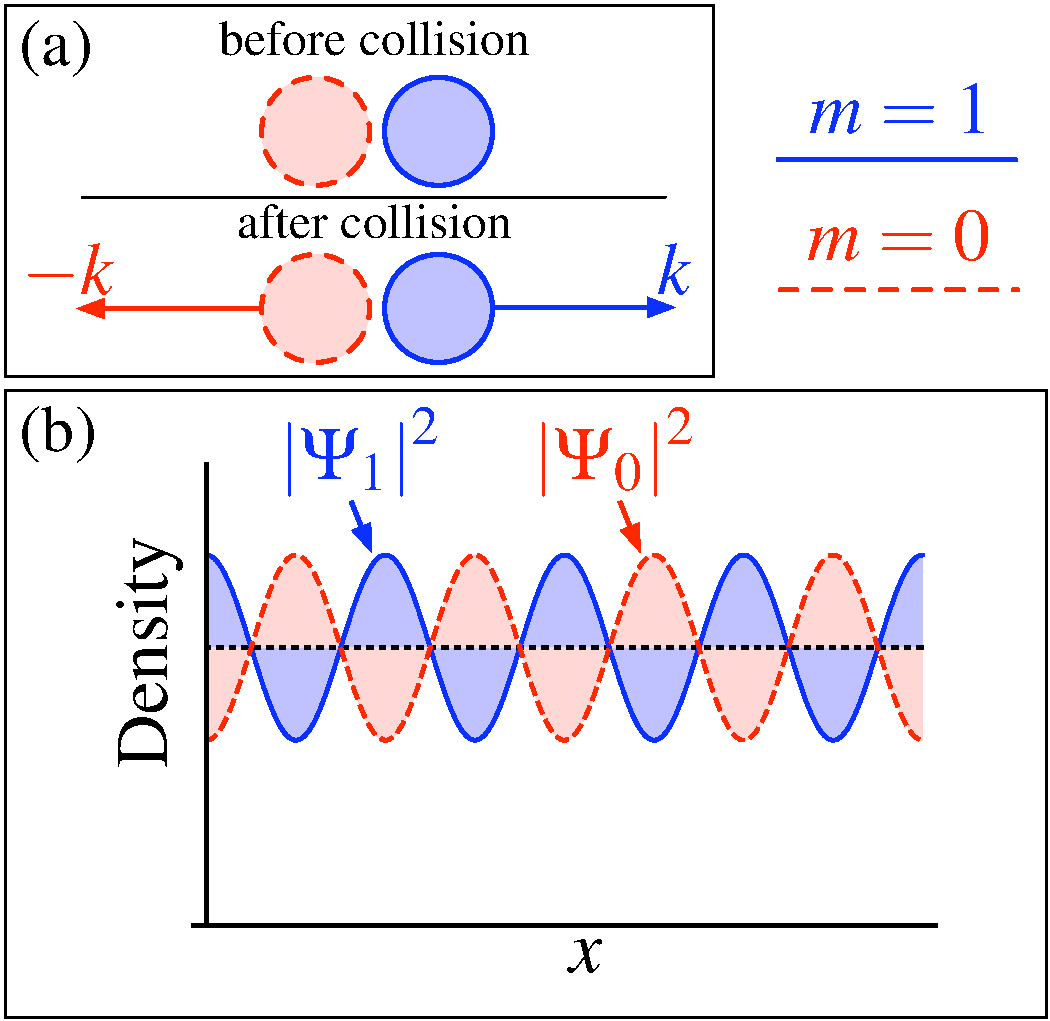
\includegraphics[width=8cm]{CollisionDiagram}
        \caption{Schematic diagram of density modulations produced by a collision
                 between stationary $m_F=0$ and $m_F=1$ atoms. Upper figure (a)
                 shows these stationary atoms scattering into oppositely-directed
                 momentum modes. Lower figure (b) shows the density grating formed
                 between the scattered atoms and the background of stationary atoms
                 in their respective states. The horizontal dotted line shows the
                 (assumed equal) background densities in both atomic states. The $x$
                 coordinate is the weak trapping dimension. The reduced mean-field
                 energy of this density grating compared to the initial uniform
                 background enables the collision shown in (a) to occur (see main
                 text).
                 \label{Peaks:CollisionDiagram}}
    \end{center}
\end{figure}

The four-wave mixing process in this experiment occurs when stationary trapped and untrapped atoms collide producing superpositions of pairs of atoms with oppositely-directed momenta in the weak trapping dimension. In the terminology of the previous section it is two $E_-$ quasiparticles that are produced. Although superpositions of pairs of atoms will be produced, in this section we will simplify our considerations by only considering one component of this superposition as shown schematically in \figureref{Peaks:CollisionDiagram}(a). The four-wave mixing process producing these atom pairs is different to the usual four-wave mixing process where two atoms with non-zero kinetic energy collide conserving kinetic energy to scatter into different momentum modes. In this experiment two stationary atoms with \emph{zero} initial kinetic energy scatter into modes with \emph{non-zero} momentum. The source of this additional kinetic energy is  a reduction in the mean field interaction energy. As will be shown, in the case of equal scattering lengths the interaction energy either is unchanged by this collision or increases. However, He* has a reduced scattering length for 0--0 collisions as compared to 0--1 and 1--1 collisions, and the interaction energy is \emph{reduced} by the collision.

To see how the interaction energy can be reduced as a result of this collision, consider the simple case of uniform, equal background fields $\Psi$ in the $m_F=1, 0$ internal states in the absence of a trapping potential. The $m_F=-1$ state is neglected as it has negligible density compared to the other states. After the collision, the mean field in each state $\Psi_i'$ is
\begin{align}
    \Psi_1' &= \psi' + \delta \psi e^{i \mathbf{k} \cdot \mathbf{x}}   \label{Peaks:MFCollisionT}\\
    \Psi_0' &= \psi' - \delta \psi e^{-i \mathbf{k} \cdot \mathbf{x}}, \label{Peaks:MFCollisionU}
\end{align}
where $\mathbf{k}$ is the wave-vector of the atoms after the collision, $\psi'$ is the mean field of the stationary atoms after the collision and $\delta \psi$ is the mean field of the atoms that have collided. These scattered atoms with momenta $\pm \hbar \mathbf{k}$ will interfere with the background stationary atoms in their respective states. This interference causes density gratings for both the trapped and untrapped internal states,
\begin{align}
    \abs{\Psi_1'}^2 &= \abs{\psi'}^2 + \abs{\delta \psi}^2 + 2 \psi'\delta\psi \cos (\mathbf{k}\cdot \mathbf{x})\\
    \abs{\Psi_0'}^2 &= \abs{\psi'}^2 + \abs{\delta \psi}^2 - 2 \psi'\delta\psi \cos (\mathbf{k}\cdot \mathbf{x}).
\end{align}
As the number of atoms in each state is unchanged, the density of each state can be rewritten in terms of the original background mean field $\Psi$ of each state as
\begin{align}
    \abs{\Psi_1'}^2 &= \abs{\Psi}^2 + \varepsilon(\mathbf{x})\\
    \abs{\Psi_0'}^2 &= \abs{\Psi}^2 - \varepsilon(\mathbf{x}),
\end{align}
where $\varepsilon(\mathbf{x}) = 2 \psi' \delta\psi \cos (\mathbf{k}\cdot\mathbf{x})$. 

The mean field interaction energy after the collision will be
\begin{align}
    \mean{\hat{H}_\text{int}} &= \sum_{i j} U_{ij} \int d\mathbf{x}\, \mean{\hat{\Psi}_i^\dagger \hat{\Psi}_j^\dagger \hat{\Psi}_j \hat{\Psi}_i}\\
                              &= U \int d\mathbf{x}\, \left(\abs{\Psi_1'}^4 + \kappa \abs{\Psi_0'}^4 + 2 \abs{\Psi_1'}^2\abs{\Psi_0'}^2\right) \\
                              &= U \int d\mathbf{x}\, \left[ (3+\kappa)\abs{\Psi}^4 + 2 (1 - \kappa) \varepsilon(\mathbf{x}) \abs{\Psi}^2 - (1 - \kappa) \varepsilon^2(\mathbf{x})\right],
\end{align}
where $U_{i j} = 4 \pi \hbar^2 a_{i j}/M$ is the nonlinear interaction strength, $a_{i j}$ is the s-wave scattering length between the internal states $i$ and $j$, $U=U_{1 1} = U_{1 0}$ and $\kappa = a_{0 0}/a_{1 1} < 1$. For atoms like Rubidium, $\kappa \approx 1$ and the interaction energy factorises to only depend on the total density, which is unchanged by the collision. However, for metastable Helium $\kappa < 1$ and the interaction energy has reduced as a result of the collision,
\begin{align}
    \Delta\mean{\hat{H}_\text{int}} &= U (1-\kappa) \int d\mathbf{x}\, \left[2 \abs{\psi'}^2\varepsilon(\mathbf{x}) - \varepsilon^2(\mathbf{x})\right] \label{Peaks:DeltaInteractionEnergy}
\end{align}
as the first term in this expression averages to zero over one period of the density grating, and the second term is always negative, indicating that the interaction energy has \emph{reduced} due to the scattering. 

Performing the integral in \eqref{Peaks:DeltaInteractionEnergy} over some volume gives,
\begin{align}
    \Delta \mean{\hat{H}_\text{int}} &= -2 U (1-\kappa) \abs{\psi'}^2 N_\mathbf{k},
\end{align}
where $N_\mathbf{k}$ is the number of atoms in the integrated volume in the $m_F=1$ state with momentum $\hbar \mathbf{k}$. Due to conservation of energy, this reduced interaction energy must be balanced by the kinetic energy of the scattered atoms,
\begin{align}
    \mean{\hat{T}_1} + \mean{\hat{T}_0} + \Delta \mean{\hat{H}_\text{int}} &= 0 = (2 N_\mathbf{k}) \frac{\hbar^2 \mathbf{k}^2}{2 M} -2 U (1-\kappa) \abs{\psi'}^2 N_\mathbf{k}, \label{Peaks:SimpleEnergyConservation}
\end{align}
where $\hat{T}_i$ is the total kinetic energy operator of the $m_F=i$ state. The $2 N_\mathbf{k}$ term in this expression comes from the $N_\mathbf{k}$ atoms in the $m_F=1$ state with momentum $\hbar \mathbf{k}$ and the $N_\mathbf{k}$ atoms in the $m_F=0$ state with momentum $-\hbar \mathbf{k}$. Solving \eqref{Peaks:SimpleEnergyConservation} for the magnitude of the resonant wavenumber $\abs{\mathbf{k}}$ and neglecting the change in the condensate density so that $\abs{\psi'}^2\approx \abs{\Psi}^2$ gives
\begin{align}
    \abs{\mathbf{k}_\text{res}} &= \frac{1}{\hbar}\sqrt{2MU\abs{\Psi}^2\left(1-\kappa\right)}.
\end{align}


Generalising this argument to consider different density backgrounds $\Psi_i$ for the $m_F=1, 0$ states yields the wave number corresponding to the energy-momentum resonance of the scattered atoms as
\begin{align}
%    \abs{\mathbf{k}} &= \frac{1}{\hbar} \sqrt{2 M U \abs{\psi'}^2(1-\kappa)}
    \abs{\mathbf{k}_\text{res}} &= \frac{1}{\hbar} \sqrt{2 M U \big(2 \abs{\Psi_1}\abs{\Psi_0} - \abs{\Psi_1}^2 - \kappa \abs{\Psi_0}^2\big)} \label{Peaks:ResonantWavenumber}.
\end{align}
This is a different expression to that obtained in the previous section \eqref{Peaks:BogResonantWavenumber}, as in this section it has been assumed that there is an equal density in both $m_F=1, 0$ excitations, an assumption not made in the previous section.

% The two expressions are equal when $\abs{\Psi_1}^2 = \kappa \abs{\Psi_0}^2$ corresponding to no disturbance of the total mean field experienced by the $m_F=0$ state

%The resonant momentum for the gratings in the numerical simulations of $\unit[1.2\times 10^6]{m}^{-1}$ is in excellent agreement with the result given by \eqref{Peaks:ResonantWavenumber} of $\unit[1.3\times 10^6]{m}^{-1}$.

\section{Full 3D calculation}
\label{Peaks:3DCalculation}

\subsection{Calculating Momentum Flux Density at the Edge of a Simulation Region}
When simulating a process the calculation region must include all of the interesting dynamics, however, unless a technique is used for removing 

without infinite calculational resources, a technique is required for 


When performing simulations the simulation region must contain the 


When performing simulations to model dynamics that occur over any significant timescale, 
